%\documentclass{beamer}
\documentclass[handout]{beamer}

\usepackage{tikz,fancyvrb,hyperref,multicol,relsize,verbatim,ulem}%,enumitem}
%\usepackage{enumitem}
\usepackage{mathrsfs,mathtools,framed}
\usepackage[T1]{fontenc}


\usetikzlibrary{shapes,arrows}


%\usetheme{Warsaw}


%\usecolortheme{beaver}


\usefonttheme{professionalfonts}
%\setbeamercolor{block}{bg=red, fg=white}
\setbeamercolor{block title}{bg=blue!25}
\setbeamercolor{block body}{bg=blue!15}


\AtBeginSection[ ] {
\begin{frame}<beamer>{ }
\frametitle{Outline}
\tableofcontents[currentsection]
\end{frame} }



\newcommand{\leqAS}{\overset{\textrm{a.s.}}{\leq}}

\renewcommand{\b}{\textbf}
\newcommand{\bX}{X}
\newcommand{\bS}{\mathbf{S}}
\newcommand{\cX}{\mathcal{X}}
\newcommand{\hJ}{\widehat{J}}
\newcommand{\cI}{\mathcal{I}}
\newcommand{\cQ}{\mathcal{Q}}
\newcommand{\hcQ}{\widehat{\mathcal{Q}}}
\renewcommand{\bar}{\overline}
\newcommand{\proj}{\mathcal{P}}
\newcommand{\cY}{\mathcal{Y}}
%\newcommand{\cS}{\mathcal{S}}
\newcommand{\cT}{\mathcal{T}}
\newcommand{\pow}{\textnormal{Pow}}


\newcommand{\bcol}[2]{{\usebeamercolor[fg]{#1} #2}}
\newcommand{\bstrc}[1]{\bcol{structure}{#1}}
\newcommand{\balrt}[1]{\bcol{alerted text}{#1}}

%\usepackage{multimedia}
\usepackage{../../mycommands}
\newcommand{\hk}{\hat{k}}
\newcommand{\cE}{\mathcal{E}}
\newcommand{\cN}{\mathcal{N}}
\newcommand{\Err}{\cE}

\newcommand*\mystrut{\vrule width0pt height0pt depth1.5ex\relax}
\newcommand{\underlabel}{\underbracket[1pt][.5pt]{\mystrut \quad\;\; \sub \quad\;\; }}


\title{Sequential Adaptive Model Selection}

\author{Will Fithian\\~\\
  {\small Joint with:}\\
  Jonathan Taylor,\\ Rob Tibshirani,\\ Ryan Tibshirani}
\date{\today}


\begin{document}


\frame{\titlepage}



\section{Sequential Model Selection}


\frame{\frametitle{Motivation: Model Selection in Regression}
  \bstrc{Given:} response $Y \in \R^n$, predictors $X_1,\ldots, X_p$
  \vskip+1em
  Run $d$ steps of LARS / LASSO / Forward Stepwise: 
  \vskip+1em
  $\quad\imp$ sequence of selected \bstrc{variables}
  $j_1,\ldots, j_d \in [p]=\{1,\ldots,p\}$
  \vskip+1em
  $\quad\imp$ sequence of \bstrc{active sets} 
  $E_k = \{j_1,\ldots,j_k\}$
  \[\emptyset \sub E_1 \sub \cdots \sub E_d\]
  $\quad\imp$ sequence of nested \bstrc{regression models} 
  \[
  M_0 \sub M_1 \sub \cdots \sub M_d
  \]
  \[
  M_k:\;Y \sim \cN_n(X_{E_k}\beta, \sigma^2 I_n)
  \]
  \bstrc{Goal:} choose $k$
  \vskip+1em
  \bstrc{Prior Work:} Taylor, Lockhart, Tibshirani, Tibshirani (2013); Loftus and Taylor (2014)
}

\frame{\frametitle{Motivation: Principal Components Analysis}
  \bstrc{Given:} data matrix $X \in \R^{n\times m}$, sample covariance
  \[
  S = \frac{1}{n-1} \sum_{i=1}^n (x_i - \bar x)^2
  \]
  Run $d$ steps of PCA:
  \vskip+1em
  $\quad\imp$ sequence of selected \bstrc{eigenvectors}
  $u_1, \ldots, u_d$
  \vskip+1em
  $\quad\imp$ sequence of nested \bstrc{Wishart models}
  \[
  M_0 \sub M_1 \sub \cdots \sub M_d
  \]
  \[
  M_k:\; (n-1)S \sim W_m
  \left(\lambda_0 I_m + \sum_{i=1}^k\lambda_i u_iu_i', 
    \;\;\;n-1\right)
  \]
  \bstrc{Goal:} choose $k$ 
  \vskip+1em
  \bstrc{Prior work:} Choi, Taylor, and Tibshirani (2014)
}

\frame{\frametitle{Motivation: Exploratory Model Selection}
  \bstrc{General Setup:} Data $Y\sim F$, $F$ unknown
  \vskip+1em
  Use $Y$ to \bstrc{adaptively} generate sequence of nested models
  \[
  M_0(Y) \sub M_1(Y) \sub \cdots \sub M_d(Y)
  \]
  \bstrc{Goal 1:} for $k \in [d]$, construct $p_k(Y)$ to test 
  \[
  H_{0,k}:\; F \in M_{k-1}
  \quad \text{ vs. } \quad
  H_{1,k}:\; F \in M_k \setminus M_{k-1},
  \]
  adjusting for selection
  \vskip+1em
  \bstrc{Goal 2:} choose smallest adequate model $M_{k_0}$
}

\frame{\frametitle{What About Cross-Validation?}
  
}

\frame{\frametitle{Which Null?}
  Regression case: Should we test \bstrc{selected model} null
  \[
  H_{0,k}:\; F\in M_{k-1} \iff 
  Y \sim \cN(X_{E_{k-1}}\beta, \;\;\sigma^2I_n)
  \]
  or \bstrc{full model} null
  \[
  \widetilde H_{0,k}:\; Y \sim 
  \cN(X_{[p]\setminus j_k}\beta, \;\;\sigma^2I_n)
  \]
  Suppose $X_1$ signal, $X_2,\ldots,X_p$ noise, $X_1$ selected at step $k=4$
  \vskip+1em
  We take \bstrc{model-centric} point of view: \\
  models $M_1,\ldots,M_3$ are incorrect
  $\imp$ want to select $M_{4}$
  \vskip+1em
  Contrast with \bstrc{variable-centric} point of view 
  (e.g., knockoffs):\\ 
  variables $j_1,\ldots,j_3$ are false discoveries
  \vskip+1em 
  Will revisit this question later...
}

\frame{\frametitle{Outline}
  \begin{enumerate}
  \item Inference for single step
    \begin{itemize}
    \item Selective $p$-values
    \item Why selected model $\gg$ saturated model
    \end{itemize}
  \item Inference for full path
    \begin{itemize}
    \item Stopping rules based on $(p_1,\ldots,p_d)$
    \item When are the $p_k$ independent?
    \end{itemize}
  \item Simulation
  \end{enumerate}
  \vspa
  Focus: \bstrc{regression} models ($\sigma^2$ known or unknown)
  \note{sigma^2 known or unknown}
}


\section{Inference for One Step}


\frame{\frametitle{Inference for Step $k$}
  At step $k$, construct valid $p_k(Y)$ to test
  \[
  H_{0,k}:\; F \in M_{k-1}(Y)
  \quad \text{ vs. } \quad
  H_{1,k}:\; F \in M_k(Y) \setminus M_{k-1}(Y),
  \]
  \bstrc{Selective $p$-value} for fixed models $(m_{k-1},m_k)$
  \[
  \P_F(p_{k,m_{k-1},m_k} \leq \alpha \mid M_{k-1}=m_{k-1},
  \;M_k=m_k) \leq \alpha, \quad \forall F \in m_{k-1}
  \]
  Combine to get $p_k(y) = p_{k, M_{k-1}(y), M_k(y)}(y)$:
  \[
  \P_F\left(p_k \leq \alpha \mid M_{k-1}, \;M_k, 
    \;F\in M_{k-1}\right) \leq \alpha
  \]
  \note{F not random, but the models and p values are}
  How to get $p_{k,m_{k-1},m_k}$?
}

\frame{\frametitle{Fixed-Question Analysis}
  Must condition on \bstrc{selection event}:
  \[
  A=\{M_{k-1}(Y) = m_{k-1}, M_k(Y) = m_k\}
  \]
  $A$ depends on selection rule
  \vskip+1em
  Regression: $A$ is typically union of polytopes
  \vskip+1em
  Often, condition on finer \bstrc{selection variable}
  \vskip+1em
  \qquad e.g., condition on signs $\rightarrow$ one polytope
  \vskip+1em
  \qquad later: condition on $M_{[k]}$ and $p_{[k-1]}$ $\rightarrow$ 
  control joint law
}

\frame{\frametitle{Regression Models}
  At step $k$ add variable $j_k$, active set $E_k = \{j_1,\ldots,j_k\}$
  \vskip+1em
  Regression models for active set $E$, variable $j\in E$:
  \begin{itemize}
  \item \bstrc{Selected model:} test $H_0:\;\beta_j = 0$ in
    \[
    M:\; Y \sim \cN(X_E\beta, \;\sigma^2I), \quad (\sigma^2 \text{ kn.       / unkn.})
    \]
  \item \bstrc{Saturated model:} test $H_0:\;\eta_{j,E}'\mu = 0$ in 
    \[
    M:\; Y \sim \cN(\mu, \;\sigma^2I), \qquad (\sigma^2 \text{ known})\qquad
    \]
  \item \bstrc{Full model:} test $H_0:\; \beta=0$ in
    \[
    M:\; Y \sim \cN(X\beta, \;\sigma^2I), \quad (\sigma^2 \text{ kn. / unkn.})
    \]
  \end{itemize}
  \note{null hypotheses nested only in selected model, 
    otherwise just seq. of hyp in the same model. However,
    saturated model tests are valid for the selected model null,
    so we do have the option.}
}

\frame{\frametitle{Selected-Model Analysis}
  Selected model for active set $E_k$:
  \[
  M_k:\;Y\mid A \sim \exp\left\{\frac{1}{\sigma^2} y'X_{E_k}\beta
    - \frac{1}{2\sigma^2}\|y\|^2 - \psi_A(\beta,\sigma^2)\right\}\; 1\{y \in A\}
  \]
%  Let $T_k$ denote suff. stats for $M_k$:
%  \[
%  T_k(y) = \left(X_{E_k}'y, \|y\|^2\right) \quad \text{ if } \sigma^2 \text{unkn.}
%  \]
%  Test is based on 
  Condition on $X_{E_{k-1}}'Y$ $\rightarrow$ tests based on
  \[
  \L_{\beta_j=0}\left( X_{j_k}'Y \mid Y\in A,\;X_{E_{k-1}}'Y, \; \balrt{\|Y\| ?}\right)
  \]
  Note:
  \begin{itemize}
  \item $M_k$ has one more suff stat than $M_{k-1}$
    \note{so we add one ss to model and then test whether it helps}
  \item $p_{k,m_{k-1},m_k}$ function of suff stats of $m_k$
    \note{not true for saturated model}
  \item $p_{k,m_{k-1},m_k}$ conditions on suff stats of $m_{k-1}$
  \end{itemize}
}

\frame{\frametitle{Selected Model vs Saturated Model}
  \bstrc{Simple setting:} $n = p = 2, X = I_2, \sigma^2=1$ known
  \vskip+1em
  $\mu = \binom{4}{4}$. First step of forward stepwise:
  \vspa
  \begin{center}
  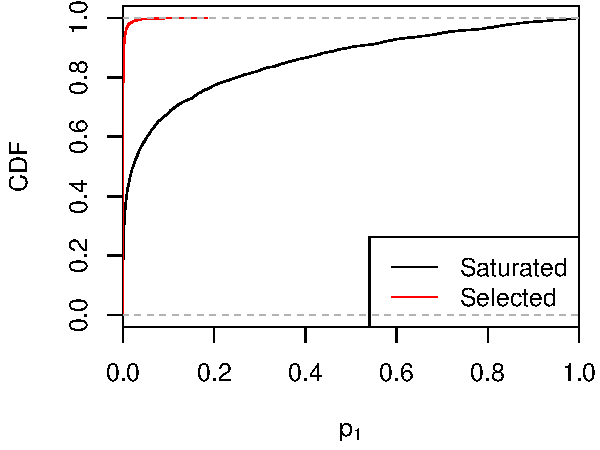
\includegraphics[width=.7\textwidth]{../figs/bivariateSelVSat.pdf}
  \end{center}
  \bstrc{Power:} 99.7\% vs. 59\% for $\alpha=.05$
}

\frame{\frametitle{Selected Model vs Saturated Model}
  \bstrc{Sel.:} $Y \sim \cN\left(\binom{\mu_1}{0}, \;I_2\right)$
  $\rightarrow$ compare to $\L_{\mu=0}(Y_1 \mid A)$
  \vskip+1em
  \bstrc{Sat.:} $Y \sim \cN\left(\binom{\mu_1}{\mu_2}, \;I_2\right)$
  $\rightarrow$ compare to $\L_{\mu_1=0}(Y_1 \mid Y_2, \;A)$
  \vspa
  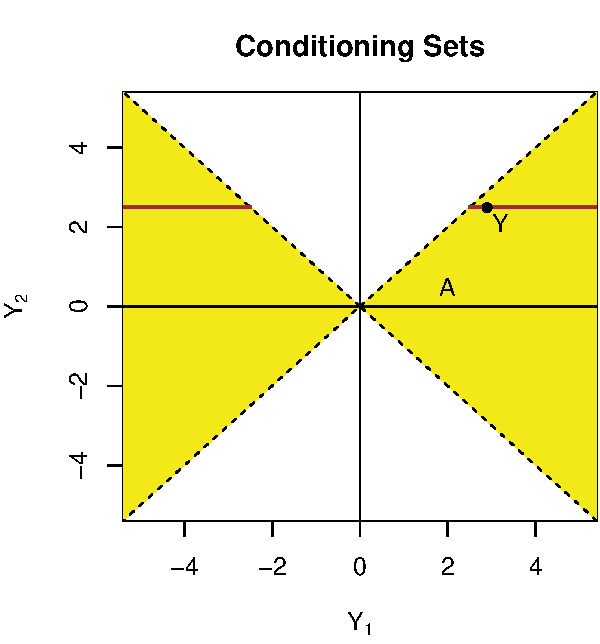
\includegraphics[width=.46\textwidth]{../figs/fullvred.pdf}
  \hspace{.03\textwidth}
  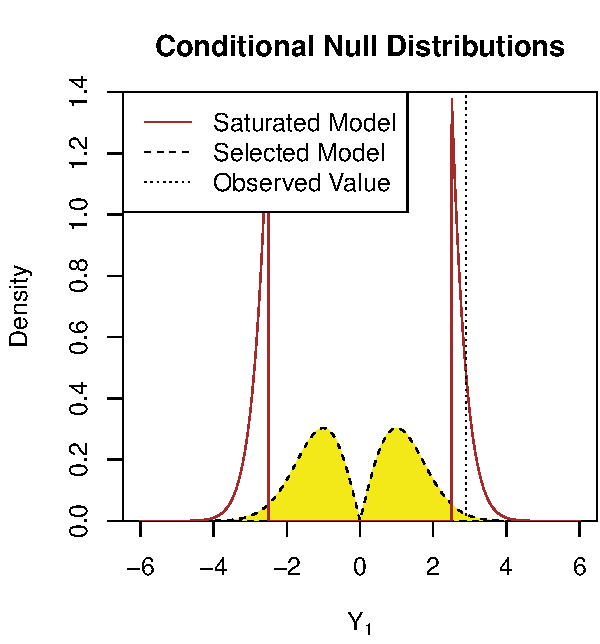
\includegraphics[width=.46\textwidth]{../figs/fullvredNulls.pdf}
}


\section{Sequential Hypothesis Testing}

\frame{\frametitle{Things to Mention}
  ``Simple Stop'' (controls FWER regardless of dependence?)
  \vskip+1em
  Options:\\
  Method $\times$ \{ Regression, Ex.Fam., Generic \}
  $\times$ \{ Saturated, Selected \}
  $\times$ Selection variable
  $\times$ Stopping rule
  $\times$ ???
}

\frame{\frametitle{Stopping Rules: Non-Adaptive Setting}
  Observe $Y \sim F$
  \vskip+1em
  Given \bstrc{fixed} sequence of nested statistical models
  \[
  M_0 \sub M_1 \sub \cdots \sub M_d % \qquad \text{(fixed, for now)}
  \]
  and $p$-values $p_k(Y), k=1,\ldots,d$ 
  \note{stochastically smaller}
  \vskip+1em
  \bstrc{Completion index:} $k_0 = \min \{k:\; F \in M_k\}$ \pause
  (first correct model)
  \vskip+1em
  \bstrc{Stopping rule:} $\hk(Y)$ estimator of $k_0$.
  \vspa
  \bstrc{Goal 2a:} Control type I errors  $(\hk(Y) - k_0)_+$
  \vskip+1em
  \bstrc{Goal 2b:} Minimize type II errors $(k_0 - \hk(Y))_+$
}

\frame{\frametitle{Strong Stop}
  G'Sell, Wager, Chouldechova, \& Tibshirani (2013)
  \[
  \hk_{S}(Y) = \max\left\{k \in \{1,\ldots,m\} :\;
    \exp\left(\sum_{i=k}^m \frac{\log p_i}{i}\right) 
    \leq \frac{\alpha k}{m}\right\}
  \]
  Controls \bstrc{familywise error rate:}
  \[
  \P\left[\hk_S(Y) > k_0\right] \leq \alpha
  \]
  under independence condition:
  \[
  (p_{k_0+1},\ldots,p_d) \mid (p_1,\ldots,p_k) 
  \sim \text{Unif}[0,1]^{d-k_0}
  \]
}



\frame{\frametitle{Forward Stop}
  G'Sell, Wager, Chouldechova, \& Tibshirani (2013)
  \[
  \hk_{F}(Y) = \max\left\{k \in \{1,\ldots,m\} :\;
    -\frac{1}{k}\sum_{i=1}^k \log(1-p_i) \leq \alpha\right\}
  \]
  Controls \bstrc{false discovery rate:}
  \[
  \E\left[\frac{(\hk_F(Y) - k_0)_+}{\hk_F(Y) \vee 1}\right] \leq \alpha
  \]
  under independence condition:
  \[
  (p_{k_0+1},\ldots,p_d) \mid (p_1,\ldots,p_k) 
  \sim \text{Unif}[0,1]^{d-k_0}
  \]
}


\frame{\frametitle{Post-Selection Inference}
  G'Sell et al. implicitly assume $M_k$ fixed for $1 \leq k \leq d$.
  \vskip+1em
  Adaptive variable selection $\imp$ \balrt{random} sequence
  \[
  M_0(Y) \sub M_1(Y) \sub \cdots \sub M_d(Y)
  \]
  Completion index $k_0(Y)$ is \balrt{random} (function of $M(Y)$)
  \vskip+1em
  $\L(p_k(Y))$ is \balrt{random} (uniform if $k > k_0(Y)$, otherwise not)
  \vskip+1em
  \balrt{NB:} $F$ is \balrt{not} random
  \vskip+1em
  What error rate \balrt{should} we control?
}


\frame{\frametitle{Post-Selection Error Rates}
  Error rate = expectation of loss $\Err(\hk(Y), k_0(Y))$
  \[
  \Err(\hk, k_0) = \left\{
    \begin{matrix}
      (\hk - k_0)_+/(\hk \vee 1) & \text{FDR}\\
      1\{\hk > k_0\} & \text{FWER}\\
      \cdots & \cdots
    \end{matrix}
  \right.
  \]
  Strongest adaptive error control guarantee:
  \[
  \E\left[\Err(\hk, k_0) \mid M_0,\ldots,M_d\right] \leq \alpha
  \]
  Implies
  \[
  \E\left[\Err(\hk, k_0) \mid k_0\right] \leq \alpha, 
  \quad \text{ and } \quad
  \E\left[\Err(\hk, k_0)\right] \leq \alpha
  \]
}

\frame{\frametitle{Post-Selection $p$-Values}
  We want \bstrc{strongest} adaptive guarantee
  \[
  \E\left[\Err(\hk, k_0) \mid M_0,\ldots,M_d\right] \leq \alpha
  \]
  for $\hk_F(p_1,\ldots,p_d)$ and $\hk_S(p_1,\ldots,p_d)$.
  \vskip+1em
  \bstrc{Goal:} Given arbitrary selection rule
  \[
  M_0(Y) \sub M_1(Y) \sub \cdots \sub M_d(Y),
  \]
  generate $p_1(Y),\ldots,p_d(Y)$ with 
  \[
  (p_{k_0+1},\ldots,p_d) 
  \mid (M_1, \ldots, M_d, \;k_0, \;p_1, \ldots, p_{k_0}) 
  \sim \text{Unif}[0,1]^{d-k_0}
  \]
  
}

\frame{\frametitle{Relating the two}
  For independent null $p$-values, condition on stuff up to $k-1$
  \begin{block}{Lemma (FTTT 2015)}
    Assume that for all $F,k,\alpha$,
    \[
    \P_F\left(p_k \leq \alpha \mid M_{[k-1]},p_{[k-1]}\right) 
    \1\{F \in M_{k-1}\} \leqAS \alpha.
    \]
    Then, 
    \[
    \P_F\left(p_{k+1}\leq \alpha_{k+1}, \ldots, p_d \leq \alpha_d
      \mid p_{[k]}, k_0(Y)=k\right) 
    \leqAS \prod_{\ell=k+1}^d \alpha_\ell 
    \]
  \end{block}
  Proof:
  \[
  \P_F\left(p_d \leq \alpha_d \mid p_{[d-1]}, k_0(Y)=k\right) 
  \leqAS \alpha_d
  \]
}

\section{Simulation: Sparse Linear Regression}

\frame{\frametitle{Generating Model}

}

\frame{\frametitle{Comparisons}

}

\frame{\frametitle{The End}
  \begin{center} 
    {\Huge Thanks!}
  \end{center}
}

\end{document}